%!TEX root = ../main.tex
\chapter{引言:基于超导量子比特与固态自旋的混合量子系统简介}
\label{cha:intro}




        自从量子理论于上世纪初被提出、建立与发展以来,对世界产生了众多深远的影响。而在1970到1980年间,一些学者开始以可设计的角度来看待与研究量子系统\cite{feynman1982simulating},这带来了一系列观念的变化,人们开始思考如何制备与设计量子系统以达到不同的目的,以及综合物理、计算机科学以及信息论来提出一些全新的问题。\cite{nielsen2002quantum}自从量子加密通信的BB84协议\cite{bennett1984quantum},量子搜索算法\cite{grover1996fast}与量子质因数分解算法\cite{shor1994algorithms}被提出后,人们看见了基于量子力学原理的计算机与通信系统能够在一些问题上达到超越经典系统的性能,进而促进了量子信息实验的进展。

        \section{混合量子系统的重要性与现有研究状况} % (fold)
        \label{sec:importance}

            基于量子力学的计算机的最基本的组成元素为量子比特。一个量子比特是一个二能级量子系统的统称。,为了满足组建量子计算机的目的,一个好的二能级系统需要可扩展,可初始化,退相干时间远大于单次操作时间,可构建任意的量子逻辑门,可被独立测量这五个条件\cite{divincenzo2000physical}。人们对许多不同的微观二能级系统进行了尝试,包括量子点\cite{loss1998quantum},离子阱\cite{haffner2008quantum},固态自旋系统\cite{gershenfeld1997bulk},超导量子比特\cite{devoret2013superconducting}以及线性光学\cite{kok2007linear}等。

            这些不同系统各自建立的量子比特有不同的特点,例如基于离子阱的量子比特有很高的操作与测量成功率,但其扩展性相对较差;超导量子比特有较好的扩展性,并且容易操作,但其退相干时间则相对较短;基于光子的量子比特则是量子通讯的最佳选择。因此,通过将不同量子系统耦合起来,分别利用他们各自的优点进行相应的操作,是量子计算与量子通信的发展趋势。本文主要关注由超导量子比特与固态自旋系统构成的混合量子系统。


            利用自旋系综作为量子存储器的想法在近十年前便开始有人提出\cite{Dutt2007,Imamoglu2009,Wesenberg2009},并且进行了相关基础实验,如自旋系综与超导微波谐振腔的耦合\cite{Schuster2010},并且能够达到强耦合的程度\cite{kubo2010},也即耦合强度超过了自旋系综以及谐振腔的衰减与退相干速率。这些实验充分说明利用自旋系综与超导谐振腔耦合这一课题的重要性与意义。另一方面,也有直接将自旋系综或是单个自旋与超导量子比特进行耦合的相关理论计算\cite{Marcos2010}与实验工作\cite{Zhu2011,Mark2013}。这篇文章主要考虑单个自旋或自旋系综与谐振腔的耦合,进而通过谐振腔再与超导量子比特进行耦合,不考虑单个自旋或自旋系综与超导量子比特的直接耦合。通过自旋与谐振腔的耦合,还可以通过谐振腔达到量子极限的测量精度\cite{Bienfait2016a}以及通过谐振腔的Purcell效应控制自旋系综的能量衰减速率\cite{Bienfait2016b},这些都是十分有意义的工作。

            由于自旋通过谐振腔中的磁场与谐振腔形成耦合,磁场的不均匀性将导致自旋与谐振腔耦合强度的不均匀性。在提高谐振腔的磁场均匀性这个方面,有相关工作通过在传输线谐振腔的基础上增加中心传输线的条数达到改善谐振腔磁场均匀性的效果\cite{Benningshof2013,Mohebbi2014},也有相关工作从改良三维谐振腔的角度出发,在保持谐振腔中磁场的均匀性的效果前提下增加磁场强度进而增加耦合强度\cite{Angerer2016}。在单个自旋与谐振腔耦合这方面,通过改进电感部分的设计,可以局域地增强磁场强度,进而增大谐振腔与单个自旋的耦合强度\cite{Jenkins2014,Eichler2017},从而可能通过单个自旋达到强耦合的程度\cite{sarabi2017prospective}。

            本文将计算并重现对传输线谐振腔磁场的仿真计算并估计自旋与传输线谐振腔的耦合强度,也从改良三维谐振腔的角度进行了仿真。另一方面,本文仿真并改进了通过重新设计谐振腔电感部分以增强耦合强度的设计,并进一步开始尝试该设计的微纳加工实现,并整理了微纳加工流程。对制备出来的器件,通过PPMS测量系统进行了测量。本文的第\ref{cha:spin_simulation}章中介绍了前文提到的多个仿真工作。对于测量系统的搭建与改进的相关内容在第\ref{cha:PPMS测量系统}章中有详细介绍,并在第\ref{cha:2_5维谐振腔的制备与测量}章中展示了改良的谐振腔的微纳加工工艺并利用搭建的测量系统对其进行了测量。在附录\ref{cha:SCQubitPrinciple}中介绍了超导量子比特的基础知识,随后在附录\ref{cha:fabrication}中包含了微纳加工各个步骤的详细流程与相关参数。测量系统搭建过程中编写的控制程序也附于附录\ref{cha:measurement_code}中供查阅。




        \section{超导量子系统与常见固态自旋系统} % (fold)
        \label{sec:qubit_and_spin}

            常见的超导量子比特由以下哈密顿量描述:
            \begin{equation}
                H_{sc} = 4 E_C (\hat n - n_g)^2 -E_J \cos \hat \phi
            \end{equation}
            其中$ E_C $与$E_J$分别为电容能量与约瑟夫森能量,两者比值的不同取值范围对应不同的超导量子比特种类,本文的工作将集中关注Transmon超导量子比特,这种量子比特对应$E_J/E_C\sim 50$的量级\cite{koch2007charge}。通过哈密顿量可以看出,超导量子比特对应非线性的谐振子,其能级非均匀分布,因而可以控制其量子态处于两个选定的本征态构成的态空间内,一般选择其基态与第一激发态,进而近似作为一个两能级系统构成量子比特。经过一系列化简,可将Transmon超导量子比特的哈密顿量写成两能级系统的标准形式
            \begin{equation}
                H_{trans} = \frac{1}{2}\hbar \omega_a \sigma_z 
            \end{equation}
            其中$ \omega_a = \sqrt{8E_JE_C}/\hbar $为基态与第一激发态的能量差对应的频率。通过将超导量子比特与平面谐振腔进行耦合,即可进行超导量子比特的操作与读取。

            自旋为很多微观粒子具有的量子特性,如电子自旋与核自旋。因为自旋与环境作用相对较弱,因此具有较长的退相干时间,是理想的存储介质。常见的自旋系统如金刚石色心(NV centers),由金刚石中一个碳原子被氮原子替代,以及相邻的一个碳原子空缺共同组成,构成一个等效的自旋为一的量子系统,如图\ref{fig:NV_centers}所示。

            \begin{figure}[h]
                \centering
                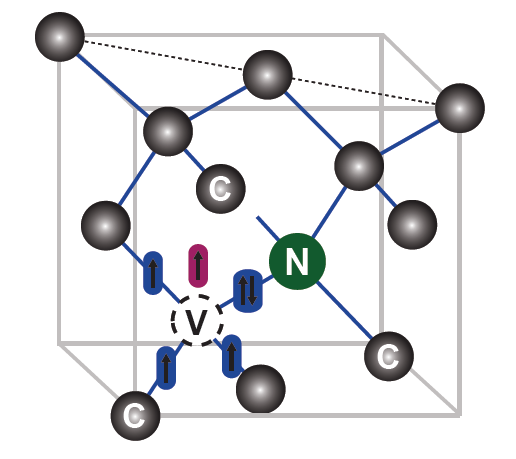
\includegraphics[width=3in]{NV.png}
                \caption{金刚石色心结构示意图,其中碳空位由V表示,氮掺杂由N表示\cite{grezes2016towards}。}
                \label{fig:NV_centers}
            \end{figure}%

            \begin{figure}[h]
                \centering
                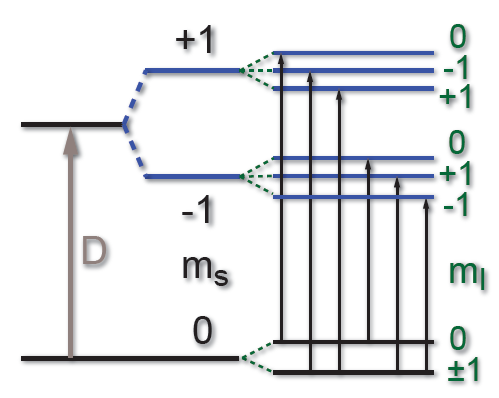
\includegraphics[width=3in]{NV_levels.png}
                \caption{金刚石色心在考虑零场劈裂与外加磁场后的能级示意图。其中$D$为零场劈裂导致的能级分裂,$m_S = \pm1$的两个态之间的能量差来源于应力与局域电场。不同核自旋量子数$m_I$的态之间的能级分裂来源于超精细相互作用\cite{grezes2016towards}。}
                \label{fig:NV_levels}
            \end{figure}

            考虑应力产生的零场劈裂以及外加静磁场后,一个金刚石色心中的自旋的简并能级发生分裂,相应的哈密顿量为\cite{grezes2016towards}
            \begin{equation}
            \label{eqn:NV_hamiltonian}
                H/\hbar = \bm S \cdot \bar{\bm D} \cdot \bm S - \gamma_e \bm B_{NV} \cdot \bm S + S \cdot \bar{\bm A}\cdot I +P I_Z^2
            \end{equation}
            其中$ \gamma_e = -g_e \mu_B /\hbar = -2\pi \times 2.8 \mathrm{MHz/Gs} $为NV电子自旋的旋磁比。$\bar{\bm D} $为零场劈裂张量,$\bm B_{NV} $为金刚石色心所处位置的磁场,$\bar{\bm A}$为超精细相互作用张量,最后一项为氮原子四极矩产生的能量项。知道了系统的哈密顿量后,即可选取两个态构成量子比特,这样近似下的哈密顿量与二能级系统的哈密顿量相同。通过将自旋与不同量子系统进行耦合,即可达到存储与读取量子信息的目的。
            




            

        \section{超导量子系统与自旋系综的耦合} % (fold)
        \label{sec:simulation_experimental_works}

            目前已有许多关于超导量子比特与固态自旋耦合的相关实验。由于自旋通过磁场与外界耦合,强度很弱,因此常采用自旋系综与平面波导谐振腔的磁场耦合,谐振腔再与超导量子比特耦合的方法\cite{grezes2016towards}。这种方法能够实现多次的存储与读取,本节将对这方面的理论工作与实验实现进行总结。

            首先考虑单个NV自旋与谐振腔的耦合。单个NV自旋与谐振腔构成的混合量子系统,可由以下哈密顿量描述
            \begin{equation}
            \label{eqn:Hamiltonian_resonator_NV}
                H = H_r + H_a + H_{int}
            \end{equation}
            其中$H_r = \hbar \omega_r a^\dagger a $为谐振腔的哈密顿量,$H_a$即由\ref{eqn:NV_hamiltonian}所描述的NV自旋自身的哈密顿量,而$H_{int}$为两个系统相互作用的哈密顿量\cite{grezes2016towards}
            \begin{eqnarray}
                H_{int} &=& - \gamma_e \bm S \cdot \bm B\\
                        &=& - \frac{\gamma_e}{\sqrt 2} [ \sigma_x \delta B_x (\bm r) + \sigma_y \delta B_y (\bm r) ](a + a^\dagger) \\
                        &=& g^* a \sigma_+ + g a^\dagger \sigma_-
            \end{eqnarray}
            其中自旋-谐振腔耦合系数
            \begin{equation}
            \label{eqn:coupling_coeff}
                g = - \frac{\gamma_e [ \delta B_x(\bm r) + i \delta B_y(\bm r) ] }{\sqrt 2}
            \end{equation}
            $\delta B $为谐振腔零场的磁场涨落。耦合系数$g$是自旋-谐振腔系统最关键的系数之一,也是我们想要通过仿真进行估算以及通过改进器件设计与制备来提高其数值的物理量。为了达到NV自旋与谐振腔中的电磁模式的强耦合,进而实现两者间量子信息的交换,我们需要$ g\gg \kappa, \gamma $,其中$ \kappa $为谐振腔的衰减率,$\gamma $为NV自旋的衰减率。对于单个自旋与二维平面波导传输线谐振腔间的耦合,$g\sim 2\pi\cdot 10 $Hz\cite{grezes2016towards},远远小于$\kappa, \gamma $的数量级,因此我们需要改进用一个自旋系综与谐振腔耦合,或者改进谐振腔的设计,来提高耦合系数。

            对于一个自旋系综与谐振腔耦合的系统,其哈密顿量为T-C模型(Tavis-Cummings model)\cite{tavis1968exact}
            \begin{equation}
                \label{eqn:T-C_model}
                H_{TC}/\hbar = \omega_r (a^\dagger a + 1/2) + \frac{\omega_s}{2} \sum^N_{j=1} \sigma_z^{(i)} + g\sum^N_{j=1}( a \sigma_+^{(j)} + a^\dagger \sigma_-^{(j)} )
            \end{equation}
            其中$ \sigma^{(j)}_{z,\pm} $为第$j$个自旋的泡利算符。所有自旋的态可以写为$\prod_{j=1,...,N} \ket{i}_j $,其中$i=g,e$。为简化记号,定义自旋系综的基态为$\ket G \equiv \ket{g_1 ... g_N} $,以及第$j$个自旋被激发的激发态$\ket {E_j} \equiv \ket{g_1...e_j...g_N} $。通过引入系综自旋算符$ \mathcal S_{X,Y,Z} \equiv \sum^N_{j=1} \sigma^{(j)}_{x,y,z}/2 $以及系综升降算符$ \mathcal S_{\pm} \equiv \sum^N_{j=1} \sigma^{(j)}_{\pm} $,上式中的T-C模型哈密顿量可简化为
            \begin{equation}
                \label{eqn:TC_model_simplified}
                H_{TC}/\hbar = \omega_r (a^\dagger a + 1/2) + \omega_s \mathcal S_z + g( a \mathcal S_+ + a^\dagger \mathcal S_- )
            \end{equation}
            基于系综的自旋算符,可以发现总自旋算符$ \mathcal S^2  = \mathcal S_X^2 + \mathcal S_Y^2 + \mathcal S_Z^2 $与整个$H_{TC}$交换,即$ \mathcal S(\mathcal S+1) $为好量子数。因此我们通过$\mathcal S^2$与$\mathcal S_Z$的共同本征态来描述自旋系综系统。整个自旋系综系统的能级如下图所示。


            
            \begin{figure}[h]
                \centering
                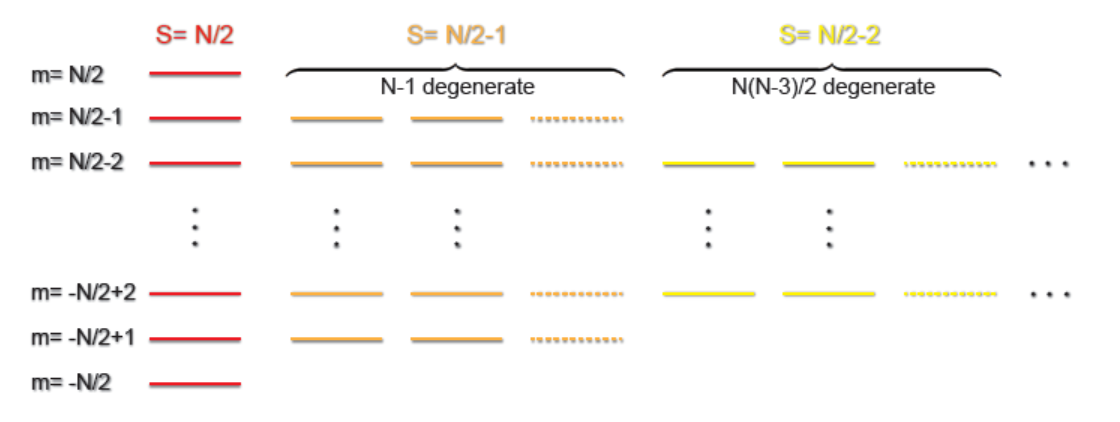
\includegraphics[width=4.5in]{NV_ensemble_levels.png}
                \caption{N个金刚石自旋构成的自旋系综的能级示意图\cite{grezes2016towards}。可以看见$\mathcal S \neq N/2 $的态均为高度简并态。}
                \label{fig:NV_ensemble_levels}
            \end{figure}




            当自旋系综从谐振腔吸收一个光子时,相应的态为$\ket B = \ket{N/2, -N/2 + 1} \equiv = \mathcal S_+ \ket G/|\mathcal S_+ \ket G| = \sum_k \ket{E_k}/\sqrt N $。其余$N-1$个单激发的激发态可写为$\ket{D_j} = \sum^{N-1}_{k=0} \exp(ijk2\pi/N)\ket{E_k}/\sqrt N $,其中$j=1,...,N-1$,且易验证$\braket{D_j|B} = 0 $。因此由能级图\ref{fig:NV_ensemble_levels}易看出所有$\ket{D_j}$对应的态均为$\mathcal S = N/2-1$,因此不可能通过$H_{TC}$与基态$\ket{G}$耦合起来。综合上述讨论,
            \begin{eqnarray}
                \bra{E,0} H_{TC} \ket{G,1} &=&(1/\sqrt N)\sum_i g = g\sqrt N\\
                \bra{D_j,0} H_{TC}\ket{G,1} &=& 0
            \end{eqnarray}
            
            
           通过上述计算可以看出,对于$N$个自旋构成的自旋系综,系综整体与谐振腔的耦合强度比单个自旋的耦合强度大了系数$\sqrt N$。
            

        % subsection simulation_experimental_works (end)



        \section{超导量子比特的制备与测量} % (fold)
        \label{sec:fabrication_characterization}
            
            建立超导量子比特与自旋的混合量子系统的基础之一是两者的成功耦合,以及超导量子比特的制备与调控。因此,本文也将对超导量子比特的理论基础\cite{schuster2007circuit,koch2007charge},制备方法\cite{krantz2010investigation,kelly2015fault}以及测量方法\cite{weber2016quantum}进行调研与总结。并以附录和文献综述的形式给出。

        % subsection fabrication_characterization (end)

